\documentclass{article}
    \usepackage{graphicx}
    \usepackage{amsmath}
    \usepackage[english]{babel}
    \usepackage[utf8]{inputenc}
    \title{Notes}
    \date{}
    \begin{document}
    \maketitle
    \section*{2659547668658713079}
\begin{tabular}{ll}
\toprule
Column & Value \\
\midrule
SourceId & 2659547668658713079 \\
right\_ascension\_euclid & 265.955000 \\
declination\_euclid & 65.871300 \\
point\_like\_prob\_euclid & 0.000006 \\
vis\_det\_euclid & 1 \\
\bottomrule
\end{tabular}

hhhjhefbefg\
\begin{figure}
    \centering
    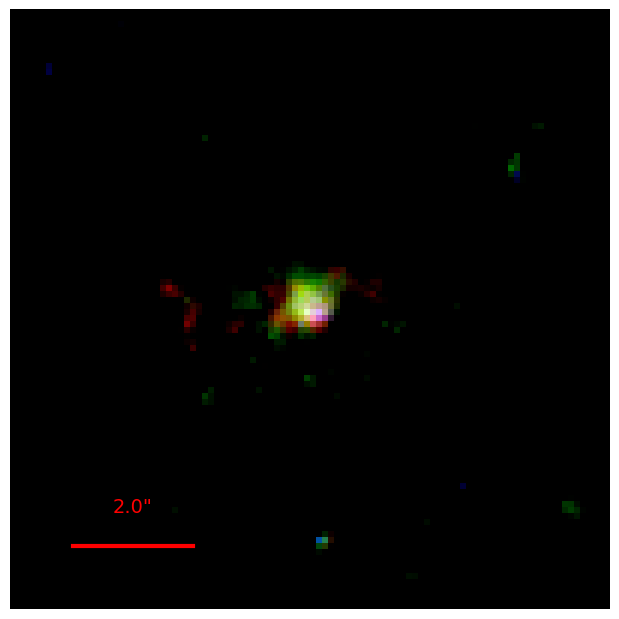
\includegraphics[width=0.5\linewidth]{2659547668658713079_Euclid_Cutout.png}
    \caption{}
    \label{}
    \end{figure}
\begin{figure}
    \centering
    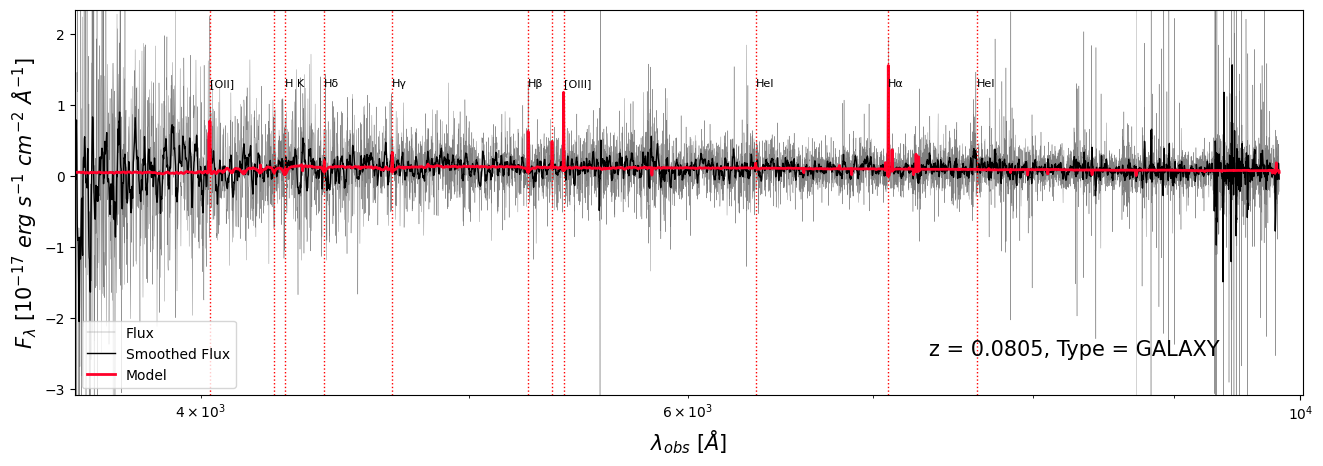
\includegraphics[width=0.5\linewidth]{2659547668658713079_DESI_spectrum.png}
    \caption{}
    \label{}
    \end{figure}

\end{document}